\documentclass{article}

% ICLR 2027 anonymous initial submission. Official style files are unmodified.
\usepackage{iclr2027_conference,times}

\usepackage[utf8]{inputenc}
\usepackage[T1]{fontenc}
\usepackage{hyperref}
\usepackage{url}
\usepackage{booktabs}
\usepackage{amsmath}
\usepackage{amsfonts}
\usepackage{microtype}
\usepackage{xcolor}
\usepackage{graphicx}
\usepackage{tabularx}
\usepackage{array}

\hypersetup{
  colorlinks=true,
  linkcolor=black,
  citecolor=black,
  urlcolor=blue
}

\graphicspath{{figures/}}

\title{Where Web Agents Go Blind:\\Missing Evidence and Answer Boundaries\\in Structurally Contained Web Content}

% Author identities are omitted for double-blind review.
\author{Anonymous Author(s)}

\begin{document}

\maketitle

\begin{abstract}
Web agents can fail because information is missing from their observation, but also because they cannot identify the boundaries of information they have read. We separate these failures in controlled web tasks. In a 1,760-trial grid, canvas removed target text from all three tested structural observations while the target region remained visible to vision. The original vision deployments nevertheless failed all 40 canvas trials: every response contained the correct token with an adjacent marker appended. Follow-ups across four deployments show that greater visual separation, labeled components, and explicit output constraints reduce this failure. An additional 880-trial study varies target values, marker strings, positions, and typography: increasing the target--distractor gap from 8 to 96 pixels reduced delimitation errors by 80--85 percentage points in every deployment and improved task success. Labeled components yielded 0/240 observed delimitation errors in the original fixed-token study and 1/240 under instance variation; the latter was a truncated target without marker inclusion. Explicit-format prompts raised varied-canvas task success from 0/80 to 57/80. The central findings are that structural observations can omit information, reading the correct token does not ensure correct delimitation, and stronger boundaries or output constraints can substantially reduce failure. We distinguish structural text reachability, target-region visibility, recovered content, and completed actions; the findings concern versioned stacks and controlled tasks rather than a universal separation threshold.
\end{abstract}

\section{Introduction}

Web agents can fail because information is missing from their observation, but they can also fail after reading the right information because they cannot identify where the requested value ends. A response such as \texttt{ALPHA-7391 | CONTROL\_READ\_VALUE\_R2} contains the correct target, yet copying the whole string produces the wrong field value. This is a delimitation failure: recognizing the target's characters is insufficient when nearby text is incorporated into the answer.

Web-agent observations may serialize the Document Object Model (DOM), expose accessibility trees, capture screenshots, or traverse browser protocols \citep{deng2023mind2web,zhou2024webarena,he2024webvoyager}. These channels can fail at different stages. Canvas text may be absent from a structural observation while remaining visible in a screenshot; a vision agent may then read that text but include an adjacent marker. Final task success alone conflates observation loss, delimitation, localization, and action execution.

Our controlled benchmark varies iframe depth and origin, shadow containment, and DOM-versus-canvas rendering while holding task semantics fixed. The primary grid identifies an observation boundary: canvas removes textual evidence from the three tested structural stacks. Archived vision responses establish a different failure: all 40 original canvas failures contain the exact target token, but also the neighboring marker. Follow-ups then vary visual separation, familiar interface layouts, component boundaries, and output instructions across four deployments.

Three findings organize the paper. \textbf{First, some observation stacks remove information:} the tested structural observations omit canvas text. \textbf{Second, visible and correctly read information does not guarantee success:} vision agents can fail to separate the target from nearby text. \textbf{Third, stronger boundaries and output constraints reduce this failure:} larger pixel gaps lower delimitation errors in every tested deployment across the familiar-layout study; the original labeled-component study yields zero observed delimitation errors; and explicit answer-format instructions improve completion. We measure target-region visibility separately from demonstrated token recovery and from successful submission.

These are capability findings about versioned stacks. Independent collectors replicate the iframe reachability null, while calibrated trials show no consistent depth gradient. Broader observation privileges also create security exposure under prompt injection \citep{roesner2026agentic}; capability to cross a boundary must be distinguished from permission to do so.

\section{Related work}

World of Bits exposed both DOM and rendered pixels \citep{shi2017worldofbits}; Pix2Act learns screenshot-to-action interaction \citep{shaw2023pix2act}. WebArena and WebArena Verified provide execution-based evaluation \citep{zhou2024webarena,elhattami2025verified}, while VisualWebArena tests multimodal tasks \citep{koh2024visualwebarena}. BrowserGym standardizes observation/action spaces and experiment management across benchmarks \citep{chezelles2025browsergym}. We complement these task-level evaluations with an independent evidence-availability score attached to a versioned collector.

SeeClick links screenshot grounding improvements to downstream GUI success \citep{cheng2024seeclick}. SeeAct identifies grounding as a bottleneck and finds hybrid HTML--visual grounding more effective than its visual-prompting alternatives \citep{zheng2024seeact}. FineState-Bench separately diagnoses localization, interaction, and exact target-state attainment \citep{ji2026finestate}. Our structural text-reachability and visual target-region-visibility scores address earlier, modality-specific questions without requiring a successful model interpretation or action. It complements, rather than replaces, such stage-wise diagnostics.

StressWeb and WebForge study controlled perturbations \citep{bai2026stressweb,yuan2026webforge}; ST-WebAgentBench includes a canvas challenge \citep{levy2026stwebagentbench}. VAF holds semantics fixed while varying visual attributes and measures changes in agent choice \citep{yu2026visualattributes}. Our separation and boundary studies instead measure target delimitation and submission alongside structural text reachability or target-region visibility. Set-of-Mark overlays labeled regions to support visual grounding \citep{yang2023setofmark}; our answer-format instruction tests a distinct intervention, without supplying an oracle region or testing a DOM cross-check.

InjecAgent and AgentDojo evaluate indirect prompt injection through external content and tool outputs \citep{zhan2024injecagent,debenedetti2024agentdojo}. Together with browser-specific isolation concerns \citep{roesner2026agentic}, they motivate separating observational capability from authorized access. Our self-authored fixtures measure capability, not adversarial robustness.

\section{Benchmark and methods}
\label{sec:methods}

\subsection{Tasks and structural axes}

The benchmark contains two deterministic tasks: reading a known value and copying a known value into a target field. Each task first passes a level-0 control consisting of a flat, single-frame, shadow-free, canvas-free page. Generated variants preserve the task instruction, correct answer and marker tokens, and external checker while changing one of four ordered axes:
\begin{enumerate}
  \item same-origin iframe depth 0--3;
  \item cross-origin iframe depth 0--3;
  \item shadow containment (none, open, closed, nested open--open); and
  \item rendering target (ordinary DOM or canvas).
\end{enumerate}
The shared level-0 condition yields 11 unique structural conditions. Pages and checkers were self-authored and deterministic; no live or authenticated service was included.

\paragraph{Fixed task content.}
Across conditions the instruction string, correct answer token, source label, and task-specific marker token are identical. The complete visible strings and layout are not byte- or pixel-identical: DOM pages place the source and prefixed marker in separate elements, whereas canvas draws the source label, value, separator, and unprefixed marker as one line. The experiment therefore holds task semantics and the two load-bearing tokens fixed while changing both representation and the boundary cues that representation provides.

\paragraph{Separation and revision studies.}
The original six-layout vision follow-up held tokens, typeface, task, and checker fixed while varying target--marker separation, with ten repeats per task and deployment ($N=240$). The revision adds 240 trials on \texttt{gpt-5.4} and \texttt{gpt-5-mini} using those same fixtures. Three familiar shells---tables, cards, and forms---cross text-box edge gaps of 8/40/96 pixels with DOM distances of zero/four parent edges ($N=1{,}440$). Visually identical DOM variants serve as negative controls; a further 240 trials use visibly distinct labeled components. A paired inline-canvas study tests explicit target formatting ($N=160$). Finally, 560 calibrated iframe trials cross four deployments, two tasks, seven conditions, and ten repeats, with positions randomized by task/repeat and matched across conditions. These arms retain eight actions and 90 seconds. An additional 880-trial instance-variation study pairs fresh tokens, markers, positions, and typography across the same four vision deployments, two tasks, and eleven layout/prompt conditions. Appendices~\ref{app:revision-design} and~\ref{app:instance-variation} specify the designs and checks.

\begin{figure}[t]
  \centering
  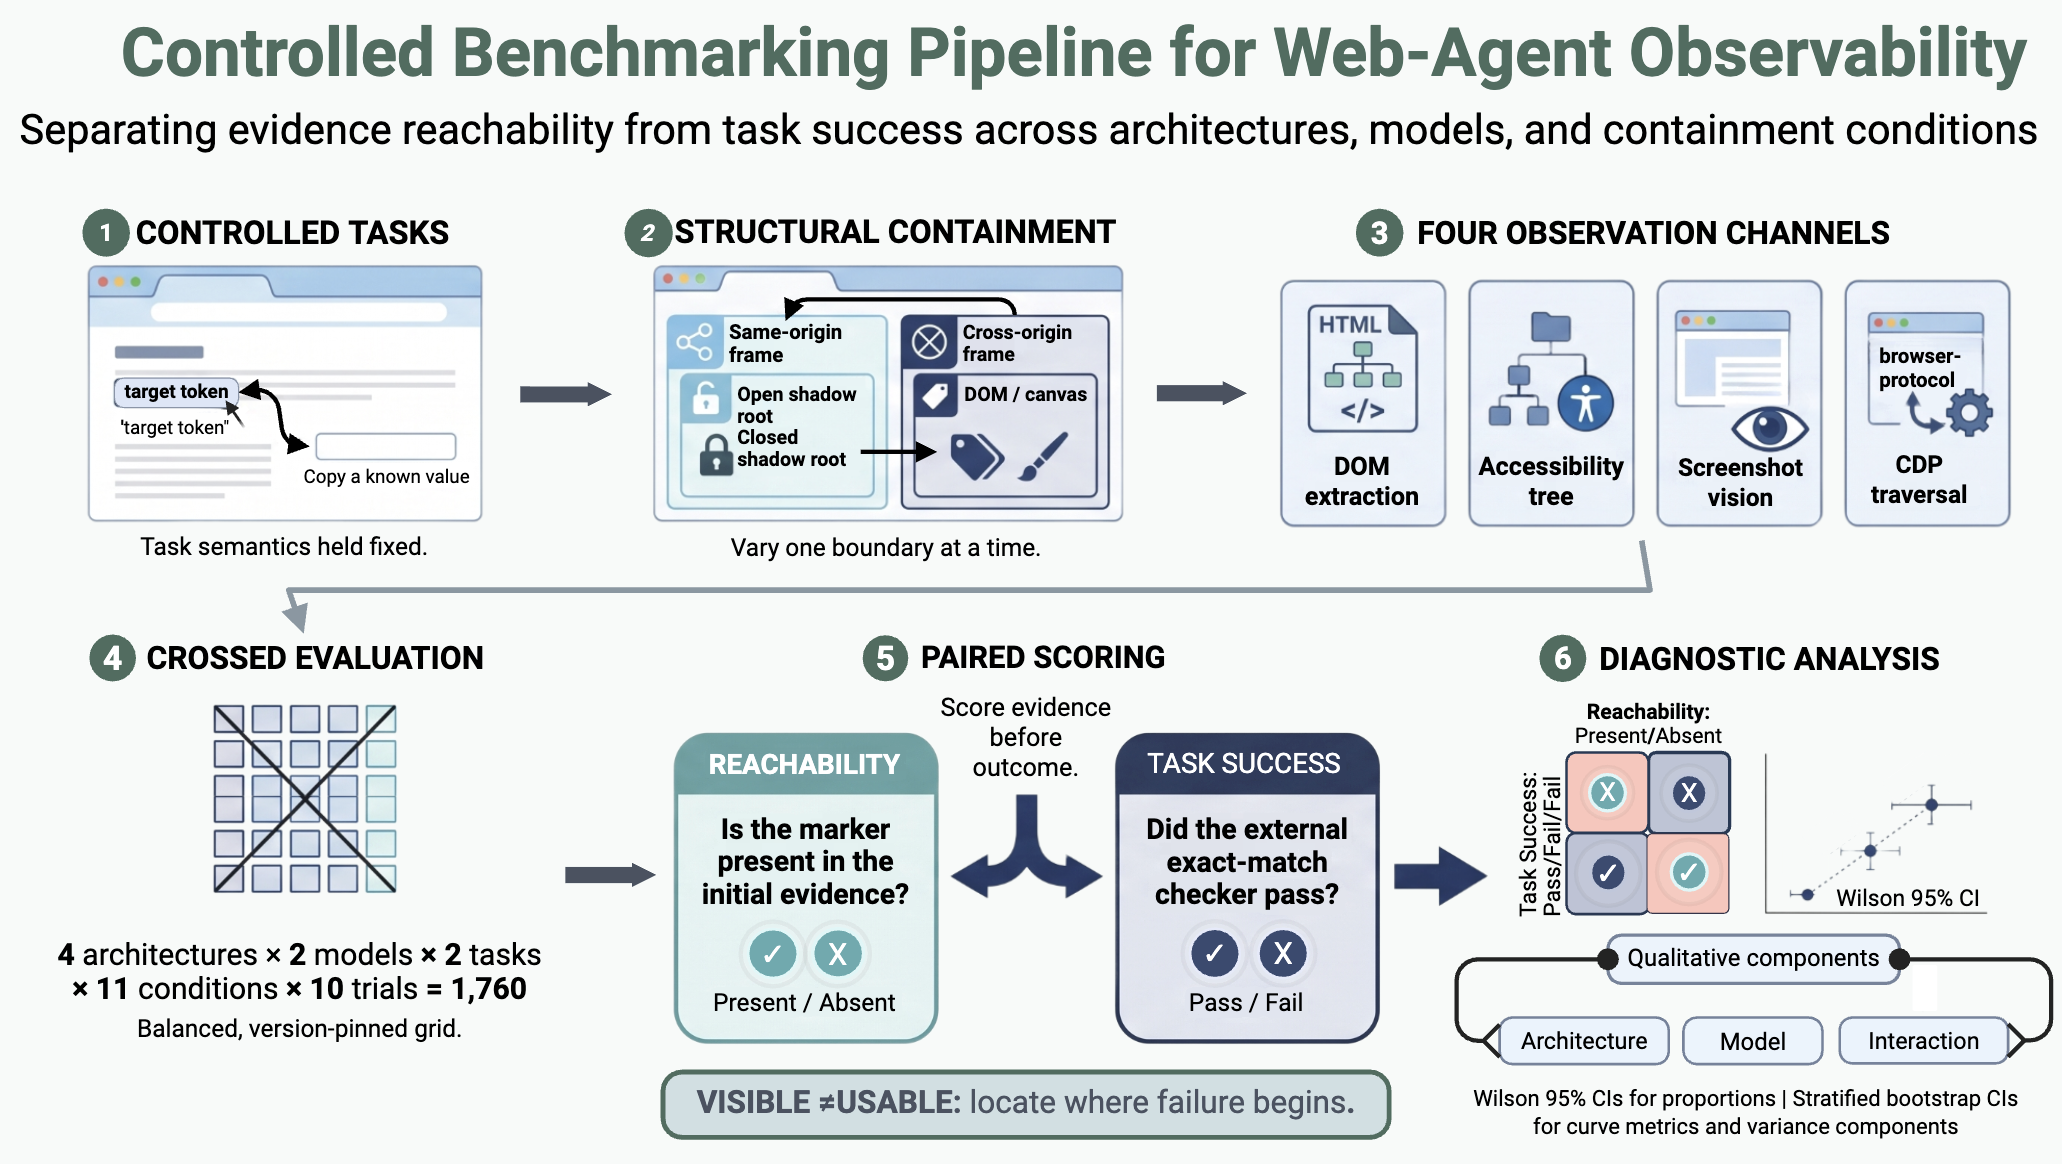
\includegraphics[width=\linewidth]{figure1.png}
  \caption{Controlled benchmarking pipeline for web-agent observability (primary grid). The schematic's reachability label denotes marker-text presence for structural observations and target-region visibility for vision; visibility does not establish legibility. Exact-match task success is scored separately.}
  \label{fig:overview}
\end{figure}


\subsection{Observation architectures and crossed models}

We evaluate four architecture classes defined by their page representation: \emph{DOM extraction} serializes page structure through an automation framework; \emph{accessibility tree} consumes the browser-computed accessibility representation; \emph{vision} receives screenshots and emits coordinate actions; and \emph{Chrome DevTools Protocol (CDP) traversal} consumes browser-level DOM snapshots and frame state. One version-pinned implementation instantiates each class (Appendix~\ref{app:implementations}). The labels therefore denote the tested pipelines rather than universal properties of every product using the same modality.

Each architecture is crossed with the same two hosted base models in the primary grid. Every task--model--condition cell contains ten valid trials, giving $4\times2\times2\times11\times10=1{,}760$ outcomes. Before the sweeps, a 48-trial control gate required all architecture--model pairs to pass both control tasks three times. In response to the small original roster, a separately versioned vision-only extension adds \texttt{foundry/gpt-5.4} and \texttt{foundry/gpt-5-mini} on the same two tasks, 11 conditions, and ten-trial allocation (440 additional valid outcomes). Run manifests preserve framework, browser, model deployment, timestamp, task revision, prompt version, and source hashes.

\subsection{Outcomes and analysis}

\textbf{Structural text reachability} indicates whether the task-specific marker appears in the initial serialized observation of a DOM, accessibility-tree, or CDP agent. This is a text-match test rescored from immutable archives without another model call.

\textbf{Target region visible} is the separate vision metric. A privileged Playwright probe searches each page frame for the benchmark marker element, target canvas, or shadow host and records whether a nonzero bounding box intersects the captured $1280\times900$ viewport. For canvas it uses \texttt{\#target-canvas}. This establishes geometric inclusion of the fixture region, not text readability or successful recognition: partial intersection alone can pass, and the probe performs neither OCR nor human legibility verification. Probe metadata never enters the model request. We therefore do not equate this metric with structural text reachability. In the original 40 failed canvas trials, exact target-token recovery in every archived response supplies separate behavioral evidence that the models read the target (Section~\ref{sec:canvas}).

\textbf{Task success} is determined by an external state checker using exact match against the correct answer. Strict equality was fixed before the sweeps; Section~\ref{sec:canvas} reports a post hoc sensitivity analysis under a relaxed criterion, because the observed canvas failures were compositional rather than substitutional.

For canvas sensitivity analyses we score the emitted answer (read) or submitted field value (copy) under three content criteria: exact match after outer-whitespace stripping; target present as a substring; and target present with the task-specific marker absent. The third permits explanatory wrapper text but rejects the observed target--marker concatenation.

We additionally record actions, input tokens, output tokens, elapsed time, and four joint outcomes formed by crossing the architecture-specific availability indicator with success. For structural observations, success conditional on unreachable text is reported only as an operational confabulation proxy, not as a claim about model intent.

\textbf{Failure coding.} For every failed vision trial we additionally code, from the archived model response and action log, where in the pipeline the failure occurred: extraction (the correct answer token is absent or altered in the response), delimitation (the correct token is present but bounded incorrectly, so the emitted string is a superset or subset of the answer), localization (the response is correct but coordinate actions target the wrong element), action execution (correct content and target, but the emitted action sequence does not reach the checked state), and abstention. Coding operates on preserved archives and requires no additional model calls.

Proportions use two-sided Wilson 95\% confidence intervals (CIs). Text-reachability and region-visibility estimates in Figure~\ref{fig:outcomes}A pool tasks and primary models within each architecture ($N=40$ per condition); both probes are model-free, but their operational meanings differ. Figure~\ref{fig:outcomes}B combines the primary and extension deployments on the matched original-layout vision-canvas cells while pooling tasks ($N=20$ per deployment); Appendix~\ref{app:modelcells} reports the underlying task--model cells ($N=10$). The four-model vision results are otherwise kept deployment-resolved, and the extension models do not enter architecture comparisons because they were not run on the three structure-based stacks. Curves use normalized trapezoidal area under the curve (AUC), total level-0-to-final drop, largest adjacent drop, and a preregistered cliff indicator. The registered variance decomposition is retained only as a confounded descriptive audit in Appendix~\ref{app:variance-audit}. Full definitions appear in Appendix~\ref{app:statistics}.

\section{Results}
\label{sec:results}

All four sweeps were complete and balanced at 440 valid outcomes per architecture. The control gate passed 48/48 trials. A provider-free rescore of the DOM and accessibility-tree archives under the final initial-page policy changed no trial labels.

\begin{table}[t]
  \caption{Overall outcomes and resource use across 11 conditions ($N=440$ per architecture). $^*$Availability denotes text reachability for structural stacks and target-region visibility for vision; these are not equivalent tests of readable text. Tokens are mean input plus output tokens; dollar cost was not archived. Success is scored by exact match; see Section~\ref{sec:canvas} for a relaxed-criterion sensitivity analysis of the vision canvas cells.}
  \label{tab:overall}
  \centering
  \small
  \begin{tabular}{lrrrr}
    \toprule
    Architecture & Availability$^*$ & Success & Actions/run & Tokens/run \\
    \midrule
    DOM extraction & 400/440 & 400/440 & 2.46 & 14,839 \\
    Accessibility tree & 400/440 & 398/440 & 2.03 & 14,927 \\
    Vision & 440/440 & 357/440 & 4.16 & 8,645 \\
    CDP traversal & 400/440 & 399/440 & 2.71 & 8,765 \\
    \bottomrule
  \end{tabular}
\end{table}

\subsection{Structural observations can remove information}

Canvas produced the sole structural text-reachability loss (Figure~\ref{fig:outcomes}A). DOM extraction, accessibility tree, and CDP traversal each fell from 40/40 on the ordinary DOM target to 0/40 on canvas (0\%; Wilson 95\% CI 0--8.8\%). The target region remained visible in 40/40 vision trials. These measurements locate the observation loss in the tested structural serializations; they do not infer readability from screenshot geometry.

Every non-canvas condition retained structural text reachability and visual target-region visibility in 40/40 trials per architecture (95\% CI 91.2--100\%). Neither iframe origin/depth nor the tested shadow containment caused measured loss. Independent Selenium frame traversal and Playwright per-frame ARIA snapshots each reached all 16 task--origin--depth cells, strengthening the iframe null across two collectors per structural modality. These versioned-stack results contradict the originally predicted cross-origin and closed-shadow cliffs, rather than establishing universal access properties.

\begin{figure}[t]
  \centering
  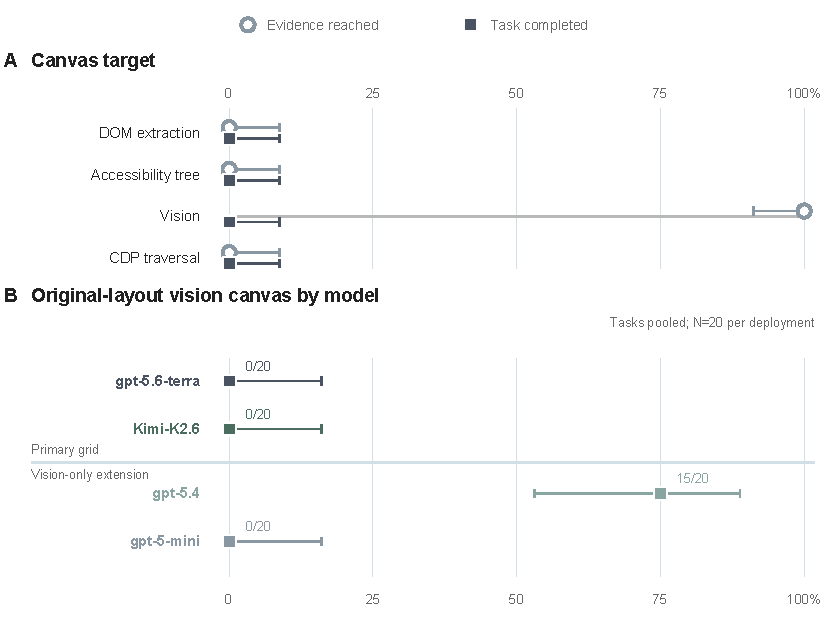
\includegraphics[width=\linewidth]{outcomes.pdf}
  \caption{\textbf{Evidence availability and task completion separate under visual observation.} (A) Primary-grid canvas estimates pool two tasks and two models ($N=40$). Structural observations had 0/40 text reachability and task success; vision had 40/40 target regions visible but 0/40 exact task success. Region visibility does not certify legibility; all 40 archived vision responses separately contained the correct token. (B) The matched original-layout vision-canvas cells combine the two primary and two extension deployments while retaining deployment-level estimates ($N=20$ each): \texttt{gpt-5.4} completed 15/20, whereas the other three completed 0/20. Whiskers are Wilson 95\% confidence intervals; Appendix~\ref{app:modelcells} gives the $N=10$ task--model cells and the full four-deployment vision grid.}
  \label{fig:outcomes}
\end{figure}

\subsection{Reading the correct token does not ensure correct delimitation}

Success closely tracked reachability for structure-based observations. Excluding canvas, DOM extraction completed 400/400 trials, accessibility tree 398/400 (99.5\%), and CDP traversal 399/400 (99.8\%); all three then completed 0/40 canvas trials. Among the 40 unreachable trials for each of these architectures, none succeeded, giving a confabulation-proxy estimate of 0\% (95\% CI 0--8.8\%). All vision target regions were visible; its corresponding nonvisible-region proxy is undefined rather than zero and is not a test of success without readable text.

Vision exposed the complementary failure mode (Figure~\ref{fig:outcomes}B): the original deployments saw all 40 canvas target regions but completed none, while completing all 120 shadow-containment trials. The original iframe success pattern was confounded by screenshot scaling and fixed absolute positions; Appendix~\ref{app:revision-design} preserves the full audit. The earlier 440-trial vision extension showed original-layout heterogeneity: \texttt{gpt-5.4} completed 15/20 canvas trials and \texttt{gpt-5-mini} 0/20. These fixed-position results motivate the separation extension and calibrated rerun below, rather than a depth claim.

\paragraph{Direct evidence of target reading and boundary failure.}
\label{sec:canvas}

Coding the 40 failed canvas trials from the two original deployments against the archived model responses and action logs, both deployments failed all 20 trials each. All 40 responses included the correct token with extra text; 0/40 produced the exact value but mislocalized the \texttt{Destination} field, 0/40 reached correct extraction and localization but failed during action execution, and 0/40 refused or abstained. Every response appended the visible control marker to the true token; in all 20 copy trials, the checker recorded that composite string in the \texttt{Destination} field. Within that preregistered roster, failure was entirely extraction---specifically, target delimitation---rather than grounding or action execution. The later \texttt{gpt-5.4} successes show that the behavior is not model-universal.

The original failure was compositional rather than substitutional: the correct token was recovered from pixels in every coded trial and was then over-included rather than replaced or hallucinated. The follow-ups below associate close visual layout with boundary errors; structural serialization can supply a boundary when tokens occupy distinct elements. Canvas is one way to remove those structural cues, not a sufficient cause of failure by itself.

\paragraph{Checker sensitivity.}
Because all 40 responses contained the target token as a substring, the canvas success rate depends jointly on rendering and on scoring strictness. We therefore report three criteria: the preregistered exact match (0/40), a permissive substring check (40/40), and an intermediate check allowing wrapper text but requiring that the target appear and the task-specific marker be absent (0/40). The last criterion rejects precisely the observed boundary error without requiring bare-token output. Thus the claim that these trials failed to delimit target from marker does not depend on choosing exact match over substring; substring instead serves as evidence that the target glyphs were read.

\subsection{Separation, component boundaries, and output constraints reduce failure}

\paragraph{The original deployments show a separation dose--response.}
For the original two deployments in the controlled follow-up, exact-match and target-without-marker criteria agreed at every level and increased monotonically from 0/40 for the inline bar, to 0/40 for two spaces, 10/40 for a 40-pixel gap, 31/40 for separate lines, and 38/40 for opposite corners. The corresponding Wilson 95\% intervals were 0--8.8\%, 0--8.8\%, 14.2--40.2\%, 62.5--87.7\%, and 83.5--98.6\%. This dose--response is specific to the original pooled deployments. The same-element DOM inline-bar control also scored 0/40 under exact and target-without-marker criteria while retaining the target substring in 40/40. Thus the original failure is not uniquely caused by canvas rendering; it is a layout-driven delimitation failure that canvas serialization cannot repair with element boundaries. Under the permissive substring criterion, the five canvas levels scored 37/40, 35/40, 29/40, 37/40, and 38/40; the nonmonotonic values reflect complete timeout/failure transcripts concentrated in Kimi copy trials rather than target--marker boundary acceptance.

\begin{figure}[t]
  \centering
  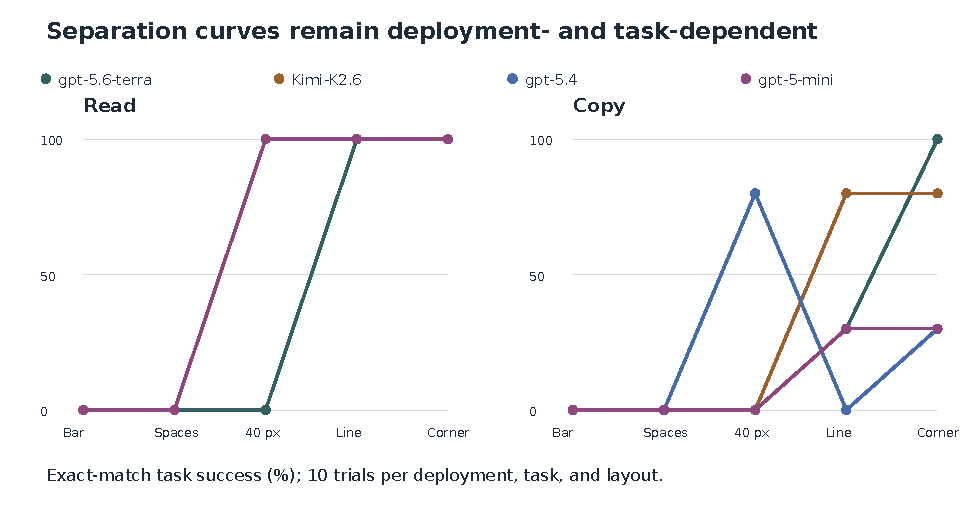
\includegraphics[width=0.92\linewidth]{canvas-separation.pdf}
  \caption{\textbf{Task success depends on separation, task, and deployment.} Exact-match success is shown separately for reading and copying, with ten trials per deployment--task--layout cell. The original two deployments and the two added deployments use the same follow-up fixtures and budgets in separate run windows. The full three-criterion estimates and Wilson intervals, including the DOM inline control, are in the artifact.}
  \label{fig:separation}
\end{figure}

\subsection{Generalization and a targeted intervention}
\label{sec:generalization}

\paragraph{The separation curve depends on the deployment and task.}
The two added deployments were tested on the same six-layout follow-up fixtures as the original deployments. Across inline bar, two spaces, 40-pixel gap, separate lines, and opposite corners, respectively, \texttt{gpt-5.4} scored 0/20, 0/20, 18/20, 10/20, 13/20. \texttt{gpt-5-mini} scored 0/20, 0/20, 10/20, 13/20, 13/20. Figure~\ref{fig:separation} retains the task split; the full three-criterion cell estimates are in the artifact. The original-layout 15/20 result for \texttt{gpt-5.4} is therefore evidence about that fixture, not a deployment-wide separation threshold.

\paragraph{Measured distance in familiar interface shells.}
Figure~\ref{fig:generalization}A reports delimitation error against measured pixel distance. Across the 360 trials per deployment, exact task success was \texttt{gpt-5.6-terra} 108/360, \texttt{Kimi-K2.6} 116/360, \texttt{gpt-5.4} 115/360, \texttt{gpt-5-mini} 41/360. Delimitation is scored from the final read answer or last attempted typed content; correct content with a failed submission is kept separate. The full estimates retain layout, task, deployment, pixel distance, and DOM separation. Because the DOM variants have the same visual appearance, their contrast is a negative control rather than a test of structural access by vision. These controlled shells broaden layout coverage but do not establish real-site generalization.

Increasing the gap from 8 to 96 pixels reduced delimitation errors by 89.2, 83.3, 79.2, and 54.2 percentage points for \texttt{gpt-5.6-terra}, \texttt{Kimi-K2.6}, \texttt{gpt-5.4}, and \texttt{gpt-5-mini}, respectively; each paired 95\% bootstrap interval excluded zero. Hidden-DOM contrasts ranged from $-2.2$ to $+3.3$ points, with all intervals including zero. Full intervals are in the artifact. Lower delimitation error alone does not imply higher task success: missing answers and failed submissions remain separate outcomes.

The natural-boundary controls use separate table columns, neighboring cards, and labeled form fields ($N=240$). Across 60 trials per deployment, exact success was \texttt{gpt-5.6-terra} 59/60, \texttt{Kimi-K2.6} 45/60, \texttt{gpt-5.4} 47/60, \texttt{gpt-5-mini} 33/60. No delimitation errors were observed in these 240 trials. Figure~\ref{fig:generalization}A places these controls at their measured mean pixel distance. They change component boundaries and labels together and therefore support a compound layout comparison, not an isolated causal effect of DOM distance.

\paragraph{Explicit target formatting.}
Figure~\ref{fig:generalization}B compares contemporaneous paired baseline and format-prompt trials. \texttt{gpt-5.6-terra} changed from 0/20 to 20/20 (+100 percentage points; paired bootstrap 95\% CI +100 to +100); \texttt{Kimi-K2.6} changed from 0/20 to 15/20 (+75 percentage points; paired bootstrap 95\% CI +60 to +90); \texttt{gpt-5.4} changed from 1/20 to 11/20 (+50 percentage points; paired bootstrap 95\% CI +35 to +65); \texttt{gpt-5-mini} changed from 0/20 to 11/20 (+55 percentage points; paired bootstrap 95\% CI +50 to +65). This tests an answer-format instruction, not an oracle region or DOM cross-check. The comparison uses its own matched baseline because the calibrated inline fixture differs in viewport and canvas width from the original 0/40 result.

\begin{figure}[t]
  \centering
  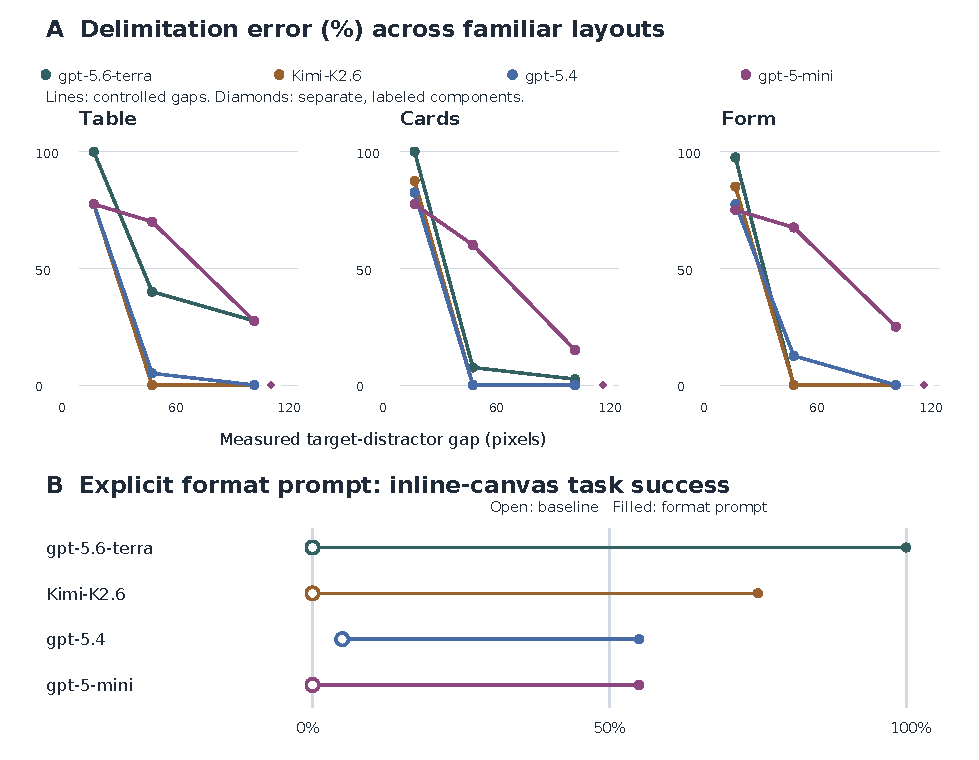
\includegraphics[width=\linewidth]{generalization-intervention.pdf}
  \caption{\textbf{Generalization by measured distance and a targeted prompt intervention.} A: delimitation-error rates in tables, cards, and forms, pooling tasks and the two visually matched DOM boundaries ($N=40$ per deployment--layout--gap point). Diamonds show separate labeled components at their measured mean distance ($N=20$); all four deployments overlap at zero observed error. B: exact task success for inline-canvas baseline (open) and explicit-format prompts (filled), with $N=20$ per deployment and arm. Cell-level Wilson intervals and paired-effect intervals are provided in the artifact.}
  \label{fig:generalization}
\end{figure}

\paragraph{Iframe depth after calibration and position matching.}
The calibrated rerun obtained all 560 allocated outcomes. Pooled over the seven conditions, read/copy success was \texttt{gpt-5.6-terra} 70/70 / 70/70, \texttt{Kimi-K2.6} 70/70 / 56/70, \texttt{gpt-5.4} 70/70 / 44/70, \texttt{gpt-5-mini} 70/70 / 10/70. Reading was 10/10 at every depth/origin cell for every deployment. Copying was 10/10 throughout for \texttt{gpt-5.6-terra}; the other deployments varied non-monotonically across depths. There is no consistent depth gradient in these outcomes. Appendix~\ref{app:calibrated} retains all task--deployment--depth cells; paired comparisons against depth zero are in the artifact. Since input screenshots are position-matched across depths, residual differences cannot be attributed to the old fixed screenshot-scale or absolute-position artifact. Ten paired repeats per cell limit sensitivity; a small or nonsignificant contrast is not evidence of equivalence. The original variance decomposition remains only a descriptive audit in Appendix~\ref{app:variance-audit}.


\subsection{Instance variation tests the failure beyond fixed strings}
\label{sec:instances}

A separately frozen 880-trial study uses ten new instances per task, varying target values, marker strings, positions, and typography while pairing instances across deployments and conditions. Increasing the gap from 8 to 96 pixels reduced delimitation errors by 80.0--85.0 percentage points across the four deployments (all paired 95\% intervals excluded zero), while exact task success rose by 66.7--80.0 points. Labeled components yielded 1/240 errors under the subset/superset endpoint: one truncated target, with no marker appended. This broad score includes character omissions and does not by itself identify a latent boundary mechanism.

On varied inline canvas, explicit-format prompts raised exact task success from 0/80 to 57/80 (11--19/20 per deployment). Appendix~\ref{app:instance-variation} reports deployment-resolved counts, paired intervals, content and submission outcomes, and design details. The failure and mitigation effects persist across these sampled synthetic instances; real-site generalization remains untested.


\section{Discussion, limitations, and future work}

Observation loss and answer-boundary failure require different remedies. Canvas removed structural text, while vision often recovered the target with nearby text appended. Separation, labeled components, and output constraints reduced failure in both fixed-token and varied-instance studies. The latter's single labeled-component error was a target truncation; correct content still did not guarantee successful submission.

These interventions do not isolate every mechanism. Labeled components change labels, geometry, and boundaries together. The format prompt excludes adjacent metadata and specifies five uppercase letters, a hyphen, and four digits; gains may reflect better delimitation, a narrower answer space, or both. The original canvas fixture also coupled rendering with close layout. Separation, DOM controls, and scoring sensitivity clarify the failure without establishing a universal visual threshold.

Two synthetic tasks, even with fresh tokens and appearances, do not establish performance on long-horizon sites or combined barriers. Added deployments cover only vision; broader architecture claims require the full roster crossed with all stacks. Independent collectors strengthen the iframe null, but ten calibrated paired repeats cannot establish depth equivalence. Resampling cannot repair the original coordinate confounds or make its variance shares causal.

Structural text reachability, target-region visibility, and demonstrated token recovery remain distinct. Visibility does not certify legibility, and response-based failure labels do not reveal latent states. Blinded coding agreed on all 40 original cases, but its single category leaves ordinary Cohen's $\kappa$ undefined (Appendix~\ref{app:failurecoding}). The structural confabulation proxy's 8.8\% upper Wilson bound cannot rule out rare unsupported success. The subset/superset endpoint can also include transcription omissions, as the new labeled-component error illustrates.

Future studies should test region prompts and structural cross-checks against both content and action outcomes \citep{yang2023setofmark,zheng2024seeact}. Selective hybrid observation may trade additional actions against context size; dollar cost and energy remain unmeasured. Real-site evaluations must separate capability from permission, comparing restricted policies under combined barriers, adversarial instructions, and sensitive decoys.

\section{Conclusion}
Some observation stacks remove information; reading a visible target does not guarantee correct delimitation; and stronger boundaries or output constraints substantially reduce the observed failure. These mitigation benefits persist across fresh tokens and appearances. Evaluations should distinguish structural text reachability, target-region visibility, recovered content, and completed actions.

\label{main:end}
\clearpage
\subsection*{AI use statement}
Generative AI assistance (OpenAI Codex) was used to implement benchmark runners, synthetic fixtures, scoring, analysis utilities, and polish figures; coordinate experiment execution; refine follow-up experimental designs; interpret archived results; and revise and format manuscript text. The historical failure-coding audit also used an independent blinded LLM coding pass, as described in Appendix~\ref{app:failurecoding}. Validation included automated scoring tests, fixture geometry and click/submit checks, archived-response inspection, paired-image hash audits, and visual inspection of the generated figures and PDF. Benchmark-model outputs are retained as experimental observations rather than treated as ground truth. The authors remain responsible for the final text, code, data, claims, citations, and artifacts.

\subsection*{Ethics statement}
All URLs and assets were self-authored synthetic fixtures. The motivating healthcare portal was never accessed or included; no personal data, third-party accounts, human participants, or crowdsourced labor were used. Broader cross-origin reach may enable data exfiltration under prompt injection, so capability should be separated from permission and paired with access controls, provenance logging, and evaluation of restricted versus unrestricted modes before deployment.

\subsection*{Reproducibility statement}
Section~\ref{sec:methods} defines the tasks and outcomes. Appendices~\ref{app:implementations} and~\ref{app:revision-design} document the versioned stacks, fixture geometry, prompts, run allocation, and coordinate checks; Appendices~\ref{app:statistics} and~\ref{app:calibrated} give statistical definitions and calibrated cells. The accompanying tables and manifests distinguish the prior 2,640-trial revision from the additional 880-trial instance-variation study; each retains its own allocation and provenance. The original anonymous repository is linked in Appendix~\ref{app:reproducibility}; original and revision run windows remain distinct.

\clearpage
\bibliographystyle{iclr2027_conference}
\bibliography{references}

\clearpage
\appendix
\section*{Supplementary Material}

\section{Implementation and run provenance}
\label{app:implementations}

\begin{table}[h]
  \caption{Version-pinned implementations used in the completed grid. Model deployment identifiers are the aliases recorded in the manifests.}
  \label{tab:implementations}
  \centering
  \small
  \begin{tabularx}{\linewidth}{lXl}
    \toprule
    Class & Implementation & Prompt/version \\
    \midrule
    DOM extraction & browser-use 0.13.7 at commit \texttt{f0aa3a8}; Chromium 1228 & \texttt{dom-no-vision-v2} \\
    Accessibility tree & Playwright 1.61.0; Chromium 1228; CDP accessibility snapshot & \texttt{ax-full-action-v3} \\
    Vision & Playwright 1.61.0 screenshot and coordinate-action runner; Chromium 1228 & \texttt{vision-coordinate-v1} \\
    CDP traversal & Playwright 1.61.0 CDP DOM-snapshot runner; Chromium 1228 & \texttt{cdp-snapshot-v1} \\
    \bottomrule
  \end{tabularx}
\end{table}

The two primary Azure AI Foundry deployments were recorded as \texttt{foundry/gpt-5.6-terra} and \texttt{foundry/Kimi-K2.6}. The vision-only extension added \texttt{foundry/gpt-5.4} and \texttt{foundry/gpt-5-mini}; its 440/440 valid outcomes are hash-bound to the primary vision resolved specification. Primary-grid execution ran from 2026-08-30 17:55:16 to 2026-08-31 02:17:28 UTC, and the provider-free reconciliation manifest was written at 02:33:59 UTC. The 2026-09-04 follow-ups have separate immutable windows: the implementation probes ran 14:38:00--14:38:04 UTC, the 240-trial separation sweep 14:51:51--15:10:19 UTC, and the 440-trial vision extension 15:28:33--16:02:50 UTC. These dates are reported separately rather than retroactively changing the primary receipts. The DOM, accessibility, vision, and CDP receipts each contain task revisions, condition and model rosters, valid-trial counts, source and result hashes, exclusions, and completion verdicts. The final primary control gate used the same four architecture classes and two models and passed all 48 required trials.

For the iframe replication, Selenium 4.48.0 recursively switched into each frame and inspected that frame's own \texttt{page\_source}; Playwright 1.61.0 independently obtained a public \texttt{aria\_snapshot} from each frame. Neither path reused browser-use's serialization or the primary accessibility runner's raw \texttt{Accessibility.getFullAXTree} call. Both reached all 16 task--origin--depth cells.

\paragraph{Revision-run provenance.} The new separation, generalization, visible-boundary, intervention, and calibrated-iframe arms contain 240, 1,440, 240, 160, and 560 valid trials, respectively (2,640 total). Recorded new-trial timestamps span 2026-09-15T18:31:00.151404Z to 2026-09-16T00:29:10.284138Z. Each arm retains its own frozen fixture source, matrix, geometry, model identifiers, and result hash. Interrupted runs inherit completed outcomes unchanged and resume only unfinished or infrastructure-failed cells. This narrative revision is based on the user-designated 18-page manuscript supplied on 2026-09-18; its merged discussion and revised AI-use statement are retained. The revision package supplies per-trial measurements and cell estimates; raw local archives retain screenshots, actions, prompts, and responses. These new artifacts are separate from the original public artifact snapshot.

\section{Model-resolved task-success cells}
\label{app:modelcells}

The headline primary-grid results remain pooled where the split is uninformative. Table~\ref{tab:structural-models} confirms that both primary deployments were at or near ceiling for every non-canvas structure-based architecture. Figure~\ref{fig:outcomes}B combines all four deployments on the matched original-layout vision-canvas cells; Table~\ref{tab:vision-model-task-cells} reports the complete four-deployment vision grid. The extension models were not run through the three structure-based agent stacks and therefore do not enter an architecture-by-model decomposition.

\begin{table}[h]
  \caption{Non-canvas task success for the three structure-based architectures, shown by model deployment. Each model column contains $N=200$ trials; the pooled column contains $N=400$.}
  \label{tab:structural-models}
  \centering
  \small
  \begin{tabular}{lrrr}
    \toprule
    Architecture & \texttt{gpt-5.6-terra} & \texttt{Kimi-K2.6} & Pooled \\
    \midrule
    DOM extraction & 200/200 & 200/200 & 400/400 \\
    Accessibility tree & 200/200 & 198/200 & 398/400 \\
    CDP traversal & 200/200 & 199/200 & 399/400 \\
    \bottomrule
  \end{tabular}
\end{table}

\begin{table}[h]
  \caption{Complete four-deployment vision iframe task-success grid. Entries are successes out of ten trials. S denotes same-origin and X cross-origin; depth 0 is the shared level-0 control and is repeated across the two blocks for comparison. The bottom four rows are the vision-only extension.}
  \label{tab:vision-model-task-cells}
  \centering
  \small
  \setlength{\tabcolsep}{3pt}
  \resizebox{\linewidth}{!}{%
  \begin{tabular}{llrrrrrrrr}
    \toprule
    Model deployment & Task & S0 & S1 & S2 & S3 & X0 & X1 & X2 & X3 \\
    \midrule
    \texttt{foundry/gpt-5.6-terra} & Copy & 10/10 & 0/10 & 10/10 & 10/10 & 10/10 & 0/10 & 10/10 & 9/10 \\
    \texttt{foundry/gpt-5.6-terra} & Read & 10/10 & 10/10 & 10/10 & 0/10 & 10/10 & 10/10 & 10/10 & 0/10 \\
    \texttt{foundry/Kimi-K2.6} & Copy & 10/10 & 10/10 & 10/10 & 10/10 & 10/10 & 10/10 & 10/10 & 8/10 \\
    \texttt{foundry/Kimi-K2.6} & Read & 10/10 & 10/10 & 10/10 & 10/10 & 10/10 & 10/10 & 10/10 & 10/10 \\
    \midrule
    \texttt{foundry/gpt-5.4} & Copy & 10/10 & 2/10 & 0/10 & 7/10 & 10/10 & 0/10 & 7/10 & 2/10 \\
    \texttt{foundry/gpt-5.4} & Read & 10/10 & 10/10 & 10/10 & 10/10 & 10/10 & 10/10 & 10/10 & 10/10 \\
    \texttt{foundry/gpt-5-mini} & Copy & 10/10 & 10/10 & 9/10 & 7/10 & 10/10 & 9/10 & 9/10 & 8/10 \\
    \texttt{foundry/gpt-5-mini} & Read & 10/10 & 10/10 & 10/10 & 10/10 & 10/10 & 10/10 & 10/10 & 10/10 \\
    \bottomrule
  \end{tabular}%
  }
\end{table}

\section{Statistical definitions}
\label{app:statistics}

For a curve with ordered rates $y_0,\ldots,y_L$, normalized AUC is the equally spaced trapezoidal area divided by $L$; total drop is $y_0-y_L$; and the largest single-level drop is $\max_{\ell}(y_{\ell-1}-y_\ell)$. The cliff ratio is the largest adjacent drop divided by total drop. Curves with total drop below 0.20 are labeled \texttt{no\_material\_net\_drop}; remaining curves are labeled \texttt{cliff} when the ratio is at least $2/3$ and \texttt{slope} otherwise. Threshold sensitivity at 0.50 and 0.75 was also computed.

Wilson intervals use the two-sided 95\% score interval. Curve-metric and variance-component intervals use a deterministic stratified nonparametric bootstrap: trials are resampled with replacement within each task--model--condition cell, and the complete statistic is recomputed for 2,000 resamples. Where a contrast is deterministic within cells, as for the canvas reachability split, the resulting interval is degenerate and carries no information about sampling variability. Curve shape for the variance decomposition is represented by level-0-minus-level rates at every nonbaseline axis level, averaged over the two tasks. A balanced two-way sum of squares partitions variation into architecture, model, and interaction shares, normalized by their sum.

New-study rates use Wilson intervals. Paired-effect intervals use 10,000 bootstrap samples of complete randomized-position repeat blocks within task strata, preserving paired conditions and the layout/gap observations sharing each position. Degenerate paired bootstrap intervals reflect no observed variation, not certainty about future trials; cell Wilson intervals remain informative at ceiling. These exploratory comparisons use no equivalence margin or multiplicity adjustment.

\section{Failure coding scheme}
\label{app:failurecoding}

Each failed vision trial is assigned exactly one category, applied in order, from the archived response text and action log:

\begin{enumerate}
  \item \textbf{Extraction---substitution}: the correct answer token does not appear in the response.
  \item \textbf{Extraction---delimitation}: the correct answer token appears, but the emitted answer is a strict superset or subset of it (for example, an adjacent visible string is appended).
  \item \textbf{Localization}: the emitted answer is exactly correct, but coordinate actions targeted an element other than the specified field.
  \item \textbf{Action execution}: content and target are both correct, but the emitted action sequence did not produce the checked state.
  \item \textbf{Abstention}: the model declined, reported that it could not find the target, or emitted no answer.
\end{enumerate}

Categories are mutually exclusive and jointly exhaustive over failed trials. Coding operates only on preserved archives and involves no additional provider calls, so it inherits the provider-free reproducibility of the rest of the analysis. Initial labels were assigned deterministically by exact-string and substring comparison against the known target and marker, then hand-checked against all 40 archived response and action records. A second coding agent independently received a randomized packet with opaque case identifiers and was blinded to model, condition, repeat, run identifier, first-coder labels, and aggregate results. It assigned all 40 cases to extraction failure, matching the first coder in 40/40 cases. Ordinary Cohen's $\kappa$ is undefined because both marginal label distributions have zero variance (expected chance agreement is 1.0); raw agreement is 100\%, and prevalence-adjusted bias-adjusted $\kappa=1.00$ is reported only as a sensitivity statistic.

\section{Recorded resource curves}
\label{app:cost}

\paragraph{Resource profiles.}

Resource use did not follow a simple ``vision is more expensive'' pattern. Vision took the most actions but used fewer tokens overall and per action (2,076 tokens/action) than DOM extraction (6,034), accessibility tree (7,338), or CDP traversal (3,230). Per-action figures are means of per-trial ratios and therefore differ slightly from the ratio of the pooled means in Table~\ref{tab:overall}. Accessibility-tree tokens per action rose most sharply with iframe depth, consistent with increasingly large serialized tree contexts. Appendix~\ref{app:cost} shows the pooled iframe-depth curve; the artifact includes the complete per-condition cost curves. Because archived responses omitted billing amounts, we report actions and tokens rather than imputing dollar cost.



\begin{figure}[h]
  \centering
  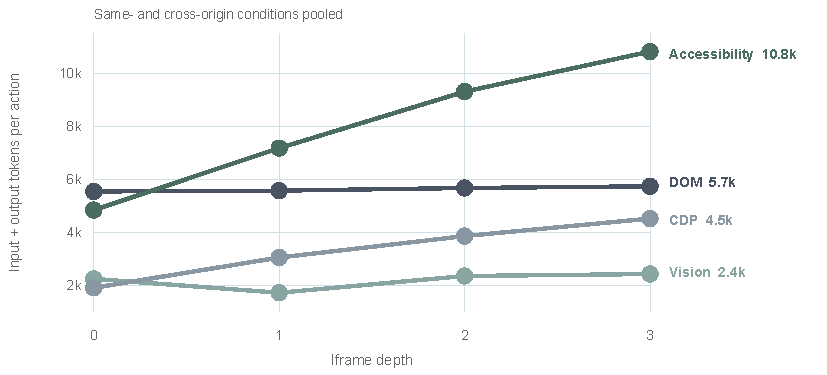
\includegraphics[width=\linewidth]{cost.pdf}
  \caption{\textbf{Serialized context grows differently across observation channels.} Lines show mean input-plus-output tokens per recorded action across iframe depth, pooling same- and cross-origin conditions, tasks, and models. The shared depth-0 control has $N=40$ per architecture; depths 1--3 have $N=80$ each. Overall actions and tokens per run are reported in Table~\ref{tab:overall}; complete per-condition estimates are included in the artifact.}
  \label{fig:cost}
\end{figure}

\section{Fixture and revision-study details}
\label{app:revision-design}
\paragraph{Fixture geometry.}
Because the canvas result below turns on visual separation between adjacent strings, we state the fixture layout explicitly. Each task page displays the target value together with a visible task-specific control marker---\texttt{CONTROL\_READ\_VALUE\_R2} for reading and \texttt{CONTROL\_COPY\_VALUE\_R5} for copying---which is present in every condition and is not part of the correct answer. In DOM conditions, the source label and value occupy one block-level paragraph, while the marker appears in a separate later paragraph in smaller text prefixed by ``Target marker:''; the copy form intervenes between those paragraphs in the copy task. In the canvas condition, a single \texttt{fillText} call draws the complete string at $(20,80)$ in a $900\times160$ canvas using 24-pixel sans-serif type, with the target and marker on the same line separated only by one space, a vertical bar, and one space (\texttt{ | }). The copy task requires writing the target value---and only the target value---into a field labeled \texttt{Destination}.

\paragraph{Visual-separation follow-up.}
To separate rendering modality from layout, a new fixture family holds task, typeface, tokens, and checker fixed while placing the target and marker (i) inline with a bar, (ii) inline with two spaces, (iii) inline with a 40-pixel gap, (iv) on separate lines, or (v) at opposite canvas corners. A sixth control renders the inline-bar string as ordinary DOM text inside one element. Both original vision deployments receive ten trials per task and layout ($N=240$). The follow-up captures at $1092\times768$, matching the high-detail image dimensions delivered to the model so screenshot and action coordinates share one space, and uses a fixed eight-action, 90-second budget. As in the primary sweep, complete timeout transcripts count as task failures; only infrastructure errors are retried and excluded. All 240 allocated outcomes were obtained with no infrastructure exclusions.


\paragraph{Deployment extension, familiar layouts, and intervention.}
A separately versioned 240-trial run extends the identical six-layout separation sweep to \texttt{gpt-5.4} and \texttt{gpt-5-mini}. We also test three self-authored interface shells---a shipment table, order cards, and a transfer form---with target--distractor text-box edge distances of 8, 40, or 96 pixels and DOM graph distances of zero or four element edges. Every combination receives ten trials per task and deployment ($N=1{,}440$ across four deployments). The DOM variants are visually matched negative controls: the vision agent cannot observe their hidden structural distinction. A 240-trial natural-boundary control places Source and Reference in separate table columns, neighboring cards, or labeled form fields; its pixel and DOM distances are measured rather than independently manipulated. A further paired study ($N=160$) compares inline-canvas baseline prompts with an explicit target-format instruction. It specifies five uppercase letters, a hyphen, and four digits, and excludes adjacent metadata without supplying the answer. The baseline and intervention share the same 730-pixel-wide canvas and $768\times768$ viewport.

Pixel distance is the minimum Euclidean edge-to-edge distance between browser text-range bounding boxes. DOM separation is the shortest parent-edge path between the elements containing the target and distractor text (zero when they share an element). Delimitation error is a nonempty candidate that contains the target with extra text or is a proper substring of the target. Candidates with other substitutions and empty candidates are recorded separately. For copying, the candidate is the last attempted typed string, while task success still requires an exact submitted value.

\paragraph{Calibrated, position-matched iframe rerun.}
A new 560-trial vision grid crosses four deployments, two tasks, seven unique depth/origin conditions, and ten repeats. Source and destination positions are randomized by task/repeat and paired across deployments, depths, and origins. Screenshots are $768\times768$ at device scale one; the prompt states those dimensions. Before model calls, pixel-center click/submit checks verify the action coordinates, and screenshots must be byte-identical across depths and origins at each paired position. These checks remove deterministic fixture scale and position differences without assuming perfect model localization. Geometry metadata remains scorer-only. All new arms retain the eight-action, 90-second budget; infrastructure failures are excluded and retried.


\subsection{Historical coordinate audit and original-layout extension}
Vision exposed the complementary failure mode (Figure~\ref{fig:outcomes}B). Its target region was visible in all 40 trials but completed none (0\%; 95\% CI 0--8.8\%), and it completed all 120 shadow-containment trials. The original iframe completion rates varied non-monotonically despite 100\% target-region visibility, but inspection of all 40 anomalous \texttt{gpt-5.6-terra} screenshots and action logs shows that this pattern is not evidence of a depth mechanism. The application programming interface's (API's) high-detail preprocessing scaled the $1280\times900$ capture to approximately $1092\times768$, while returned coordinates were executed in the original viewport. At depth 1, all 20 first copy clicks landed at $y=224$--$226$, in the 12-pixel gap between the destination label and field. At depth 2, the same biased coordinate happened to land inside the associated label and focused the input, producing an accidental recovery. The depth-3 read target was fully visible, but each of the two condition-specific screenshots elicited the identical mis-transcription \texttt{AI PHA-7391} in all ten repeats. Repeats therefore sampled model behavior on identical pixels and fixed absolute positions. Appendix~\ref{app:modelcells} retains the observed cells for transparency, but we treat them as a coordinate-runner audit and make no depth claim from them.

The two-deployment vision extension completed all 440 allocated trials with 440/440 target regions visible. Combined with the matched primary vision cells in Figure~\ref{fig:outcomes}B, it shows that the original canvas failure is not universal across models: \texttt{gpt-5.4} completed 15/20 original-layout canvas trials, whereas \texttt{gpt-5-mini} completed 0/20, matching the two original deployments' 0/20 each. The pooled four-model canvas rate is therefore 15/80, but the deployment-resolved result is primary because pooling masks this heterogeneity. Across all 11 conditions, \texttt{gpt-5.4} completed 169/220 trials and \texttt{gpt-5-mini} 189/220. Their model--task--condition cells (Appendix~\ref{app:modelcells}) remain position-sensitive: for example, \texttt{gpt-5.4} copy success was 2/10, 0/10, and 7/10 at same-origin depths 1--3 while its read success was 10/10 throughout. The broader roster demonstrates model heterogeneity but does not rehabilitate a depth interpretation of fixed-position fixtures.



\section{Instance-variation design}
\label{app:instance-variation}
A separately frozen allocation crosses four vision deployments, two tasks, ten fresh instances per task, and eleven conditions ($N=880$). Each repeat generates a new five-letter/four-digit target token, an independent 12-character reference suffix, a new absolute position, and a sampled font family, font size, and line height. The same task--repeat instance is paired across every deployment and condition. Table, card, and form shells each use an 8-pixel gap, a 96-pixel gap, or separate labeled components; inline canvas uses baseline and the existing explicit-format prompt. There is no generic-instruction arm. The two canvas prompts see the same pixels.

Targets retain five uppercase letters, a hyphen, and four digits; markers have the form \texttt{REF\_} followed by twelve uppercase letters/digits. Positions are sampled from $x=18$--65 and $y=60$--130 pixels. Font families are Arial, Verdana, or Georgia, and natural-layout text sizes are 15, 16, or 17 pixels (canvas adds four pixels). Shared natural-layout text rows use line heights of 1.2, 1.35, or 1.5; labeled components and canvas retain their own line layout. Ten instances are generated independently for each task, then reused across the matched conditions, rather than treated as independent at every layout.

Before provider calls, browser text-range or canvas text-metric boxes must lie fully inside a calibrated $768\times768$ viewport. The 8- and 96-pixel natural-layout gaps are verified; copy fixtures pass pixel-center click/type/submit checks. Geometry is scorer-only and does not enter model requests. These checks establish target-region visibility, not OCR or human-verified legibility. Screenshots, prompts, model responses, actions, instance parameters, fixture source, and checksums are archived. Execution uses eight actions and 90 seconds per trial. Timeouts and model failures count; infrastructure errors are excluded and retried without changing the allocated instance.

The primary content endpoint is delimitation error, scored from the final read answer or last attempted typed string. Exact candidate content, exact submitted success, missing answers, substitutions, and target-token presence are retained separately. Task success uses the recorded exact answer or submitted field value, independently of the runner's final status. A copy trial that already submitted the correct value remains a checked success if the runner later times out or fails to finish; terminal status is retained separately. Cell estimates use Wilson intervals; exploratory paired contrasts resample whole task-stratified instance blocks, preserving the three layouts sharing each instance. This tests robustness within the sampled synthetic tasks and token family, not real-site generalization or a universal visual threshold. Joint instance variation does not isolate separate causal effects of font, marker vocabulary, or absolute position.
% BEGIN COMPLETED RESULTS

\subsection{Completed instance-study results}
All 880 allocated trials were obtained across 20 unique task--instance blocks. All target and distractor text boxes passed viewport checks. Infrastructure errors accounted for 0 excluded attempts. All model failures and timeouts remain in the denominators.

\begin{table}[ht]
\centering\small
\caption{Instance variation: delimitation errors in familiar shells and exact task success on inline canvas. Shell counts pool three layouts and two tasks ($N=60$ per deployment and arm); canvas counts pool tasks ($N=20$).}
\label{tab:instance-results}
\begin{tabular}{lrrrrr}
\toprule
& \multicolumn{3}{c}{Delimitation errors} & \multicolumn{2}{c}{Canvas task success} \\
Deployment & 8px & 96px & Labeled & Baseline & Format \\
\midrule
\texttt{gpt-5.6-terra} & 55/60 & 6/60 & 1/60 & 0/20 & 19/20 \\
\texttt{Kimi-K2.6} & 51/60 & 0/60 & 0/60 & 0/20 & 15/20 \\
\texttt{gpt-5.4} & 48/60 & 0/60 & 0/60 & 0/20 & 12/20 \\
\texttt{gpt-5-mini} & 49/60 & 0/60 & 0/60 & 0/20 & 11/20 \\
\bottomrule
\end{tabular}
\end{table}

\begin{table}[ht]
\centering\small
\caption{Paired instance-study effects in percentage points (treatment minus baseline), with task-stratified instance-block bootstrap 95\% intervals. Gap and labeled contrasts measure delimitation error; format measures task success.}
\begin{tabular}{lrrr}
\toprule
Deployment & 96px minus 8px & Labeled minus 8px & Format minus baseline \\
\midrule
\texttt{gpt-5.6-terra} & $-81.7$ [$ -90.0, -73.3$] & $-90.0$ [$ -96.7, -81.7$] & $+95.0$ [$ +85.0, +100.0$] \\
\texttt{Kimi-K2.6} & $-85.0$ [$ -93.3, -75.0$] & $-85.0$ [$ -93.3, -75.0$] & $+75.0$ [$ +55.0, +90.0$] \\
\texttt{gpt-5.4} & $-80.0$ [$ -88.3, -71.7$] & $-80.0$ [$ -88.3, -71.7$] & $+60.0$ [$ +45.0, +75.0$] \\
\texttt{gpt-5-mini} & $-81.7$ [$ -88.3, -75.0$] & $-81.7$ [$ -88.3, -75.0$] & $+55.0$ [$ +50.0, +65.0$] \\
\bottomrule
\end{tabular}
\end{table}

\paragraph{The single labeled-component error.}
The only labeled-component output classified as delimitation was a copy trial in the card layout: \texttt{gpt-5.6-terra} submitted \texttt{ZZBH-1585} instead of \texttt{ZZZBH-1585}. The fixed scorer includes proper substrings in the delimitation endpoint, so this one-character omission is retained without relabeling. No labeled-component candidate included its reference marker. The observation is compatible with a transcription omission and does not establish an answer-boundary error by itself.
\paragraph{Content and completion remain distinct.}
The machine-readable cell tables retain each task, layout, deployment, and arm, with Wilson intervals for all endpoints. Across the three natural-layout arms, correct candidate content / exact task success / missing-answer counts were: \texttt{gpt-5.6-terra} 108/180 / 108/180 / 0/180; \texttt{Kimi-K2.6} 98/180 / 97/180 / 29/180; \texttt{gpt-5.4} 94/180 / 94/180 / 33/180; \texttt{gpt-5-mini} 111/180 / 84/180 / 20/180.
No-answer outcomes and substitutions remain distinct from delimitation; zero observed delimitation is not proof of zero risk. Instance blocks, rather than model calls or individual layout rows, are the units of bootstrap resampling. Full paired intervals and cell counts are included in the accompanying analysis.


\section{Registered variance decomposition: descriptive audit}
\label{app:variance-audit}

The registered decomposition assigned 100\% of the historical availability-indicator curve-shape variance to architecture. That indicator pooled structural text reachability with visual region visibility, so this share is not a modality-equivalent evidence measure. Task-success shares were architecture 48.7\% (95\% CI 43.0--54.9\%), model 13.9\% (11.2--17.0\%), and interaction 37.4\% (31.7--43.1\%). These reproducible summaries describe the original stacks, not causal architecture, model-family, or depth effects. Structure-based agents were near ceiling outside canvas, leaving nearly all non-deterministic variation in vision cells affected by coordinate-scale and absolute-position confounds. Resampling identical screenshots cannot remove that bias. The original-layout extension's 15/20 versus 0/20 canvas contrast broadens deployment coverage, but a vision-only extension cannot support a balanced architecture--model decomposition. That comparison requires calibrated, position-matched fixtures and the complete model roster crossed with all architectures.

\begin{figure}[t]
  \centering
  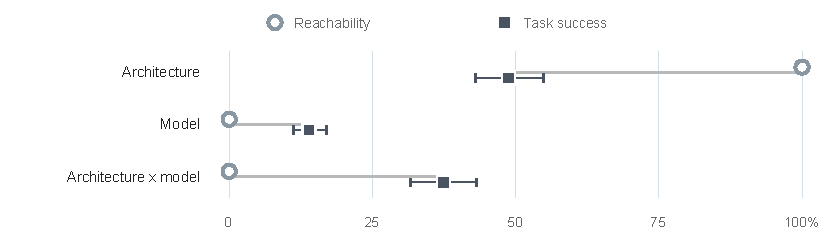
\includegraphics[width=\linewidth]{variance.pdf}
  \caption{\textbf{Registered decomposition of the original grid, retained as a runner audit.} The archived ``Reachability'' label combines structural text reachability and visual target-region visibility, which are operationally different measures. Points show each component's share of the balanced two-way sum of squares; horizontal whiskers are stratified-bootstrap 95\% intervals. Post hoc inspection identified coordinate-scale and absolute-position confounds in the vision cells that supply nearly all non-deterministic variation, so these shares are not interpreted as causal architecture, model-family, or depth effects.}
  \label{fig:variance}
\end{figure}


\section{Calibrated iframe cells}
\label{app:calibrated}
The table reports the new calibrated and position-matched study. It does not replace the archived original cells in Table~\ref{tab:vision-model-task-cells}. S and X denote same- and cross-origin fixtures. The shared depth-zero cell is repeated for readability.

\begin{table}[h]
\centering
\small
\caption{Calibrated vision task success: successes out of ten trials per cell.}
\begin{tabular}{llrrrrrrrr}
\toprule
Deployment & Task & S0 & S1 & S2 & S3 & X0 & X1 & X2 & X3 \\
\midrule
\texttt{gpt-5.6-terra} & Copy & 10/10 & 10/10 & 10/10 & 10/10 & 10/10 & 10/10 & 10/10 & 10/10 \\
\texttt{gpt-5.6-terra} & Read & 10/10 & 10/10 & 10/10 & 10/10 & 10/10 & 10/10 & 10/10 & 10/10 \\
\texttt{Kimi-K2.6} & Copy & 10/10 & 9/10 & 7/10 & 8/10 & 10/10 & 5/10 & 9/10 & 8/10 \\
\texttt{Kimi-K2.6} & Read & 10/10 & 10/10 & 10/10 & 10/10 & 10/10 & 10/10 & 10/10 & 10/10 \\
\texttt{gpt-5.4} & Copy & 8/10 & 5/10 & 4/10 & 6/10 & 8/10 & 6/10 & 7/10 & 8/10 \\
\texttt{gpt-5.4} & Read & 10/10 & 10/10 & 10/10 & 10/10 & 10/10 & 10/10 & 10/10 & 10/10 \\
\texttt{gpt-5-mini} & Copy & 1/10 & 2/10 & 3/10 & 0/10 & 1/10 & 2/10 & 1/10 & 1/10 \\
\texttt{gpt-5-mini} & Read & 10/10 & 10/10 & 10/10 & 10/10 & 10/10 & 10/10 & 10/10 & 10/10 \\
\bottomrule
\end{tabular}
\end{table}
All calibrated iframe geometry, initial screenshots, and click/submit checks are archived. Depth effects are reported as paired success-rate differences from depth zero, with bootstrap intervals in the artifact. The comparisons are exploratory; no equivalence margin was specified. Generalization availability is established from the independent text-range geometry checks; the original runner's legacy reachability selector does not identify the new field containers.
The calibrated leaf fixtures use a 360-by-44-pixel destination field and a new matched presentation. The original large-target field was at least 56 pixels high. This study estimates depth contrasts within the new fixtures; it does not isolate the effect of coordinate correction on historical success rates.
\section{Natural-boundary fixture examples}
\label{app:fixtures}
\begin{figure}[h]
\centering
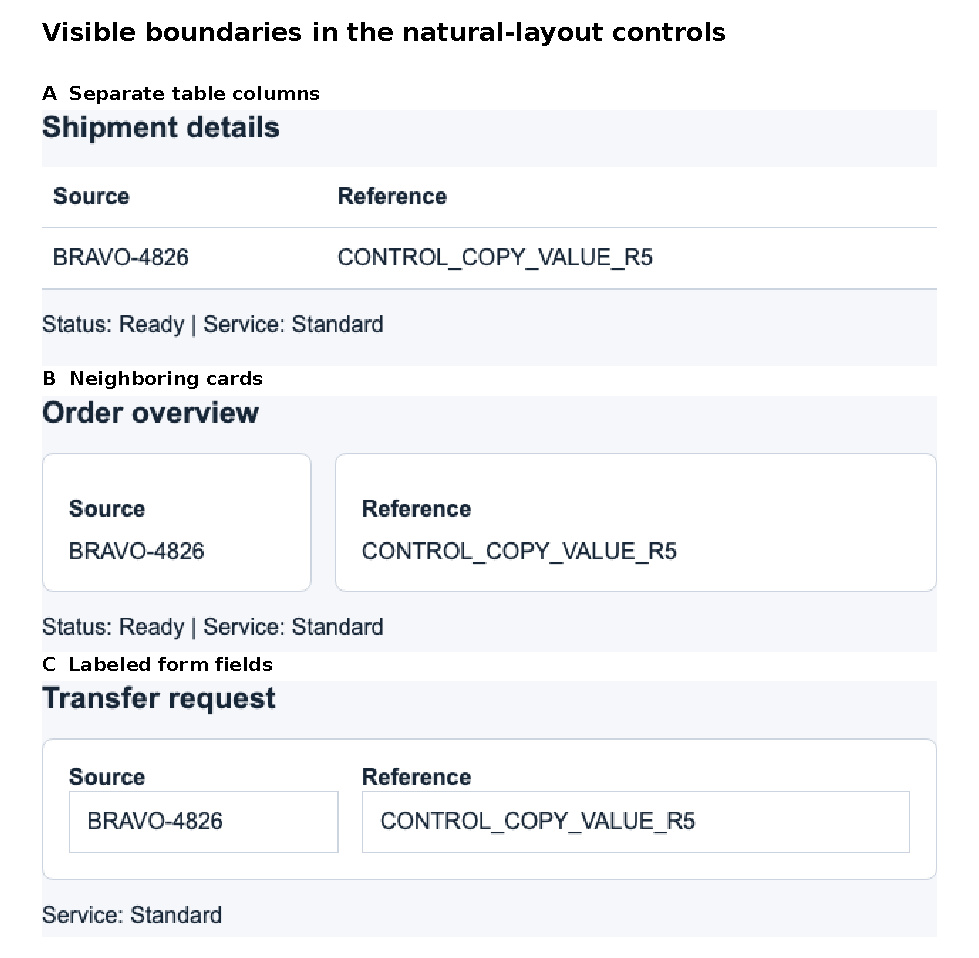
\includegraphics[width=0.65\linewidth]{natural-fixtures.pdf}
\caption{Crops of the archived copy-task fixtures for the natural-boundary control. Source and Reference occupy separate columns, cards, or labeled fields. Tokens remain fixed; pixel distances and shortest DOM parent-edge paths are measured for every fixture. The complete viewport also includes the Destination form.}
\label{fig:natural-fixtures}
\end{figure}

\section{Artifact access and reproduction requirements.}
\label{app:reproducibility}

The anonymous repository is linked at \url{https://anonymous.4open.science/r/web-agents-go-blind-D87C/}. The revised reproducibility distribution integrates the additional 880-trial instance-variation study with the earlier evidence: frozen allocations, fixture source, per-trial measurements, raw screenshot/request/response/action archives, and provider-free analysis. Its compact archive restores the full evidence with checksum verification; the reproduction driver regenerates and checks the reported tables. The distribution is prepared for the repository; availability at the hosted URL depends on publishing this revision.

The repository includes a lossless compact archive, a reconstruction script, and step-by-step reproduction instructions. Using Python 3.12 and the supplied pinned analysis dependencies, readers can reconstruct the archived files and regenerate the statistical results and result figures without browser installation or provider calls. Reconstruction verifies every restored file against its original SHA-256 checksum. Rerunning the live experiments additionally requires Chromium, the runner dependencies pinned in the lockfile, and access to the corresponding hosted model deployments. API credentials are supplied through environment variables and are excluded from the artifact.

\end{document}
